
\ifdefined\COMPLETE
\else
    \input{./preambule-sacha-utf8.ltx}
    \begin{document}
\fi


\subsection{Composition de fonctions}

\begin{tabular}{lllll}
Soit & $f$ : & $\R$ & $\longrightarrow$ & $\R$ \\
& & $x$ & $\longmapsto$ & $f\left(x\right)$ \\
Soit & $g$ : & $\R$ & $\longrightarrow$ & $\R$ \\
& & $x$ & $\longmapsto$ & $g\left(x\right)$ \\
\end{tabular}

\vspace*{.3cm}

On lit « g rond f » la fonction noté $g \circ f$.  \\

La fonction $g \circ f$ est définie par : \\

\begin{tabular}{llll}
$g \circ f$ : & $\R$ & $\longrightarrow$ & $\R$ \\
& $x$ & $\longmapsto$ & $g \circ f\left(x\right) = g\left[f\left(x\right)\right]$ \\
\end{tabular}

\vspace*{.3cm}

\subsubsection{Exemple}

\begin{tabular}{lllll}
Soit & $f$ : & $\R$ & $\longrightarrow$ & $\R$ \\
& & $x$ & $\longmapsto$ & $f\left(x\right) = 2x - 3$\\
Soit & $g$ : & $\R$ & $\longrightarrow$ & $\R$ \\
& & $x$ & $\longmapsto$ & $g\left(x\right) = x^2 + 5x - 7$ \\
\end{tabular}

\vspace*{.3cm}

1) Déterminer $g \circ f$.

\begin{tabular}{lllll}
$g \circ f$ : & $\R$ & $\longrightarrow$ & $\R$ \\
& $x$ & $\longmapsto$ & $g \circ f\left(x\right) = g\left[f\left(x\right)\right]$ \\
\end{tabular}

\begin{tabular}{lll}
$g \circ f\left(x\right)$ & $=$ &$g\left(2x - 3\right)$ \\
& $=$ & $\left(2x - 3\right)^2 + 5\left(2x - 3\right) - 7$ \\
& $=$ & $4x^2 - 12x + 9 + 10x - 15 - 7$ \\
& $=$ & $4x^2 -2x -13 $ \\
\end{tabular}

\vspace*{.3cm}

Donc $g \circ f\left(x\right) = 4x^2 -2x -13$. \\

2) Déterminer $f \circ g$

\begin{tabular}{lll}
$f \circ g\left(x\right)$ & $=$ &$f\left(x^2 + 5x - 7\right)$ \\
& $=$ & $2x^2 + 10x - 14 - 3$ \\
& $=$ & $2x^2 + 10x - 17 $ \\
\end{tabular}

\vspace*{.3cm}

Donc $f \circ g\left(x\right) = 2x^2 + 10 - 17$ \\

\textbf{Remarques}

$g \circ f \neq f \circ g$, car pour tout $x \in \R, g \circ f(x) \neq f \circ g\left(x\right)$ \\

Ici, $D_f = D_g = \R$.

\newpage

\vspace*{-1cm}

\subsubsection{Exercice musclé}

\begin{tabular}{lllll}
Soit & $f$ : & $\R$ & $\longrightarrow$ & $\R$ \\
& & $x$ & $\longmapsto$ & $f\left(x\right) = \dfrac{1}{x-1}$\\
Soit & $g$ : & $\R$ & $\longrightarrow$ & $\R$ \\
& & $x$ & $\longmapsto$ & $g\left(x\right) = \sqrt{x+3}$ \\
\end{tabular}

\vspace*{.3cm}

1) Déterminer $D_f$ et $D_g$. \\

Pour $D_f$ : il ne faut pas que $ x - 1 = 0 \Longleftrightarrow x = 1$. \\

D'où $D_f = \R \setminus \lb 1 \rb = \left]-\infty \; ; \; 1 \right[ \cup \left]1 \; ; \; + \infty \right[$. \\

Pour $D_g$ : il faut que $x + 3 \geqslant 0 \Longleftrightarrow x \geqslant -3$. \\

D'où $D_g = \left[-3 \; ; \; + \infty \right[$. \\

2) Déterminer $D_{g \circ f}$ puis la fonction $g \circ f$. \\

\begin{tabular}{llll}
$g \circ f$ : & $\R$ & $\longrightarrow$ & $\R$ \\
& $x$ & $\longmapsto$ & $g \circ f\left(x\right) = g\left[f\left(x\right)\right]$ \\
\end{tabular}

\vspace*{.3cm}

Il ne faut pas que $x = 1$ et il faut que $f\left(x\right) \geqslant -3$. \\

$\dfrac{1}{x-1} \geqslant -3 $ \\

$\dfrac{1}{x-1} + 3 \geqslant 0$ \\

$\dfrac{1 + 3x - 3}{x-1} \geqslant 0$ \\

$ \dfrac{3x - 2}{x-1} \geqslant 0$ \\

\begin{tikzpicture}
\tkzTabInit[lgt=3,espcl=2]
{ $x$  /1,
$3x - 2$ /1,
$x - 1$ /1,
$\dfrac{3x-2}{x-1}$ /1}
{$ - \infty $ , $\dfrac{2}{3} $ , $1$ , $ + \infty $}
\tkzTabLine{ , - , z , + , t , + }
\tkzTabLine{ , - , t , - , z , + }
\tkzTabLine{ , + , z , - , d , + }
\end{tikzpicture}

\vspace*{.3cm}

D'où $D_{g \circ f} = \left]-\infty \; ; \; \dfrac{2}{3}\right]\cup\left]1\; ; \; +\infty\right[$. \\

\begin{tabular}{lllll}
Il vient que $g \circ f$ : & $\R$ & $\longrightarrow$ & $\R$ & \\
& $x$ & $\longmapsto$ & $g \circ f\left(x\right) $ & $= g\left[f\left(x\right)\right]$ \\
& & & & $=g\left(\dfrac{1}{x-1}\right)$ \\
& & & & $= \sqrt{\dfrac{1}{x-1} + 3}$ \\
& & & & $= \sqrt{\dfrac{3x-2}{x-1}}$ \\ 
\end{tabular}

\newpage

3) Déterminer $D_{f \circ g}$ puis la fonction $f \circ g$. \\

\begin{tabular}{llll}
$f \circ g$ : & $\R$ & $\longrightarrow$ & $\R$ \\
& $x$ & $\longmapsto$ & $f \circ g\left(x\right) = f\left[g\left(x\right)\right]$ \\
\end{tabular}

\vspace*{.3cm}

Il faut que $x \geqslant -3$ \\

Il ne faut pas que $g\left(x\right) = 1$ \\

\begin{tabular}{lll}
$g\left(x\right) = 1$ & $\Longleftrightarrow$ & $\sqrt{x+3} = 1$ \\
& $\Longleftrightarrow$ & $x+3 = 1$ \\
& $\Longleftrightarrow$ & $x = -2$ \\
\end{tabular}

\vspace*{.3cm}

Donc $D_{f \circ g} = \left[-3 \; ; \; -2 \right[ \cup \left]-2 \; ; \; +\infty \right[$. \\

\begin{tabular}{lllll}
Il vient que $f \circ g$ : & $\R$ & $\longrightarrow$ & $\R$ & \\
& $x$ & $\longmapsto$ & $f \circ g\left(x\right) $ & $= f\left[g\left(x\right)\right]$ \vspace*{.3cm} \\
& & & & $=f\left(\sqrt{x+3}\right)$ \vspace*{.3cm} \\
& & & & $= \dfrac{1}{\sqrt{x+3} - 1}$ \vspace*{.3cm} \\
& & & & $= \dfrac{\sqrt{x+3} +1}{\left(\sqrt{x+3} - 1\right)\left(\sqrt{x+3}+1\right)}$ \vspace*{.3cm} \\ 
& & & & $= \dfrac{\sqrt{x+3} +1}{x+2}$ \vspace*{.3cm} \\ 
\end{tabular}


\ifdefined\COMPLETE
\else
    \end{document}
\fi